\documentclass[11pt]{article} % use larger type; default would be 10pt
\usepackage{graphicx,amsmath} % support the \includegraphics command and options
\usepackage{color}

\newcommand{\andyc}[1]{[{\color{red}\sc Andy comment: {\tt #1}}]}

\oddsidemargin=0.25in
\evensidemargin=0.25in
\textwidth=6in
\textheight=8.75in
\topmargin=-.5in
\footskip=0.5in

\title{NCAA working summary}
 \author{The Lemanski Sports Analytics Group}        
\begin{document}
\maketitle

\section{Introduction}
 Every March, millions of people take to an American tradition, filling out an NCAA tournament bracket.  Typical strategies include listening to so-called experts or following one's intuition, although the rise in sports analytics and the popularity of sites such as Nate Silver's fivethirtyeight.com are increasing the use of data-driven methods.  With this work we review analytic approaches to forecasting NCAA tournament games and introduce our modeling framework designed to capture matchup effects.   Many common methods for predicting outcomes assess overall team strength using ranking based metrics.  In addition to quantify overall team strength, our methodology provides a data-driven approach to assess team by team match ups and address statements of the form: \emph{"Team Y is a tough draw for team X due to their tempo, size, athleticism, three point shooting, ect.."}.  The essence of of the matchup effects is to discern the existence and magnitude of team-by-team match ups.  While there certainly is a high degree of uncertainty involved in predicting outcomes and a small number of games for evaluation, we demonstrate the efficacy of our matchup effects.  We predicted Duke would lose.  THE END
\subsection{Common Prediction Methods}
Many commonly used methods or models include a seeds based approach or using one of several rankings systems: Sagarin, Pomeroy, ESPN BPI, ect..
%%%%%%%%%%%%%%%%%%%%%%%%%%%%%%%%%%%%%%%%%%%
\section{Popular Methods}  This section reviews several existing
\subsection{Rating Based Methods} Sagarin, Pomeroy, ect...
\subsection{Ensemble Methods}
\subsection{538 methodology}
\subsection{Wisdom of the Crowds?}
%%%%%%%%%%%%%%%%%%%%%%%%%%%%%%%%%%%%%%%%%%%
\section{Data}
For many traditional bracket competitions predictions only need to be a binary result (i.e. win or lose); however, there are competitions for which probabilistic predictions  are required.  Furthermore, this provides a sensible framework for evaluating various loss functions and computing risk for various prediction schemes.  Hence, we restrict our focus to methods that return a probability of a team winning any matchup.
\subsection{Modeling Framework}
One interesting dilemma involves whether the outcomes should be modeled in a binary sense (win or loss) or rather should a continuous metric such as the point spread be used.  In theory, point spread provides a means for eliciting the relative strength of one team, although as any basketball fan can attest to the final score is often not indicative of how close the game was.  A common strategy is for the trailing team to foul in the closing moments of the game, which can often result in a two point deficit turning into a ten point loss.  For this reason, we scrape scores with 2 minutes left in the game \andyc{I think this can be done}.  A comparison of these three data aggregation methods is used on cross-validated data from... \andyc{hmm... I wonder if there is a way to tune/transform point spread to control for blowouts...}
\subsection{Common Ratings Components} wins, losses, strength of schedule...

\subsection{Other influential factors} home court, height, ect...
\subsection{Model Specification}
The general form for a linear model for point spread follows below:
\begin{eqnarray}
Y_{ij} = X_{ij} \beta + \epsilon_{ijk}
\label{eq:generic}
\end{eqnarray}
where $X_{ij}$ corresponds to the difference in predictors for teams $i$ and $j$ and $\epsilon_{ijk} \sim N(0,\sigma^2).$ 
%%%%%%%%%%%%%%%%%%%%%%%%%%%%%%%%%%%%%%%%%%%
\section{Decision Theory - Optimal Strategies}
\subsection{Probabilistic Forecasting}
\subsection{proper scoring rules}
\subsection{Strategy: Min Risk or Max Expected Earnings?}
\andyc{ The entire process could be simulated using the historical probs of seed X vs. seed Y, this would give some range on the ideal (oracle) solution in which the probs are known}
%%%%%%%%%%%%%%%%%%%%%%%%%%%%%%%%%%%%%%%%%%%
\section{Model: Nearest-Neighbor Matchup Effects}
When listening to sports broadcasters, claims of the following type are often made \emph{Team X is a tough matchup for team Y due to their ... }.  There are two ways to consider this statement: (1) the overall team strength of Team X will be problematic for Team Y or (2) Team X has certain tendencies above and beyond their team strength that will pose difficulties for Team Y.  For the first case models of the type Equation \ref{eq:generic} will account for the matchup.  However, if the second case is present we need a different approach to analytically quantify whatever characteristics may pose difficulties for a given team.  This approach is called the Nearest-Neighbor Matchup Effect and provides a means for capturing team level characteristics.  For instance, a glance inside the crystal ball would have revealed that Duke might struggle with a team like Mercer due to...  The matchup effects is a three step procedure: (1)  the typical model as in Equation~\ref{eq:generic} is fit, (2) for each matchup, past opponents most similar to the current matchup are identified, and (3) an adjustment is introduced that accounts for past performance against similar teams. 
\subsection{Matchup Effects}
The general form for the matchup effects model follows below:
\begin{eqnarray}
Y_{ij} = X_{ij} \beta + \rho( N_i(j)_k-N_j(i)_k) + \epsilon
\label{eq:ME}
\end{eqnarray}
where $X_{ij}$ coresponds to the difference in predictors for teams $i$ and $j$ and $ N_i(j)_k$ corresponds to the residual for the k nearest neighbors of $i's$ opponents to team $j$.  In other words, the second term adjusts the expected outcome based on match ups with similar teams.
\andyc{clean up notation}
\subsection{Choosing Neighbors}
There are a multitude of ways to select the neighbors.  In particular one needs to consider what variables to consider for selecting neighbors, how should those variables be weighted if at all, and how many neighbors should be selected. \andyc{Great Application for BAVA: given a set of information the users can identify similar teams which can then important variables can then be identified}  
\subsection{Tuning $\rho$}
The natural support of $\rho$ would be between zero and one.  The interpretation of the extreme points is rather intuitive - with $\rho = 0$ Equation~\ref{eq:ME} reverts to Equation~\ref{eq:generic} and with $rho = 1$ the entire residual for similar teams is retained.
%%%%%%%%%%%%%%%%%%%%%%%%%%%%%%%%%%%%%%%%%%%

\section{Evaluation}
\begin{figure}[h]
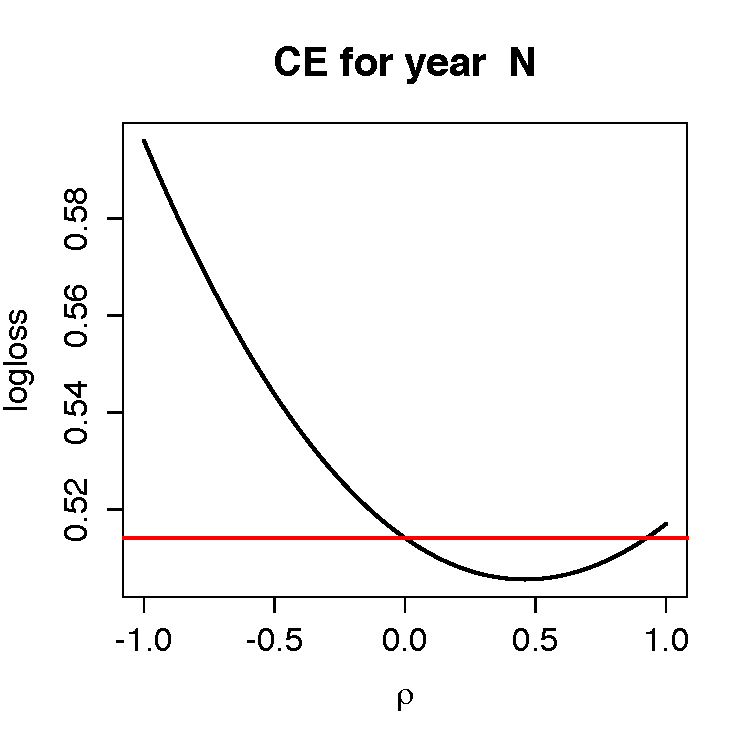
\includegraphics[width=1\textwidth]{Sample_ME.pdf}
\caption{Log loss for range of $\rho$ values}
\end{figure}
%%%%%%%%%%%%%%%%%%%%%%%%%%%%%%%%%%%%%%%%%%%
\section{Inference on Transitivity}
The transitive property states if $A>B$ and $B>C$ then $A>C$.   In terms of basketball consider:
\begin{eqnarray}
P_{A,B} > 0.5 \quad \& \quad P_{B,C} > 0.5 \rightarrow P_{A,C} > 0.5
\label{eq:trans}
\end{eqnarray}
, where $P_{I,J}$ is the probability of team I defeating team J.  Then Equation \ref{eq:trans} can be considered a transitive property on basketball match ups.  That is if team A is expected to beat team B and team B is expected to beat team C, then team A should also defeat team C.  Any sort of rank based approaches would assume this transitive ordering, home court effects non-withstanding.  Note these are probabilities not true outcomes, due to the parity in basketball inferior teams can and often do defeat stronger teams.  Nevertheless, our modeling approach can determine if the strengths of a given team present difficulties for a specific team resulting in the transitive property not necessarily holding.
%%%%%%%%%%%%%%%%%%%%%%%%%%%%%%%%%%%%%%%%%%%

\section{Evaluation}
%%%%%%%%%%%%%%%%%%%%%%%%%%%%%%%%%%%%%%%%%%%

\section{Discussion}
\end{document}
